% Short study briefing for the EPR generation-time research.  Compile with: tectonic briefing.tex
% Numbers marked interim come from an unfinished run and will be replaced by the full report.
\documentclass[10.5pt,a4paper]{article}
\usepackage[margin=20mm]{geometry}
\usepackage[T1]{fontenc}
\usepackage{booktabs,array,amsmath,xcolor,float,caption,hyperref,tikz}
\hypersetup{colorlinks=true,urlcolor=blue,linkcolor=black}
\captionsetup{font=small,labelfont=bf}
\setlength{\parindent}{0pt}\setlength{\parskip}{5pt}
\newcommand{\code}[1]{\texttt{\detokenize{#1}}}
\definecolor{demand}{HTML}{2a78d6}\definecolor{guard}{HTML}{b9b8b1}\definecolor{hit}{HTML}{1baf7a}\definecolor{fail}{HTML}{eb6834}
\title{\vspace{-12mm}EPR Generation Time and Dynamic Pre-generation:\\ Study Briefing}
\author{BTP, IIT Guwahati}
\date{1 November 2026, written while the experiments are running}
\begin{document}
\maketitle
\vspace{-6mm}
\noindent\textbf{Status.} The experiments are not finished. Results marked \emph{interim} can change. The full report comes later.

\section*{1. The question}
On-demand generation (ODG) creates an EPR pair when a request needs it, so the request waits for it.
Dynamic is the compiler-driven strategy: it uses the known future requests to create the pair earlier,
so the request can find it ready.
\textbf{The idea under test:} if generating a pair takes longer, ODG suffers more, so Dynamic should look better.
This study asks what the generation time really is, which parameters change it, and when Dynamic gains from it.

\section*{2. The baseline}
Every experiment changes only one or two things from this baseline.

\begin{table}[H]\centering\small
\begin{tabular}{@{}llp{7.2cm}@{}}\toprule
Parameter & Baseline & Meaning \\\midrule
Architecture & 4$\times$4 mesh, 16 cores & 12 slots per core: 8 data and 4 communication \\
Memories per core, $M$ & 3 or 4 & communication memories available for EPR pairs \\
Compiler memories, $C$ & $M-1$ & at most this many prepared pairs per core; one slot stays for the ODG fallback \\
Memory efficiency & 0.95 & chance a memory emits its photon \\
Detector efficiency & 0.95 each & chance each of the two detectors fires \\
BSM success rate & 0.5 & linear-optics limit \\
Fibre & 0.025 m, 0.0002 dB/m & loss is negligible at this length \\
Success per attempt, $p$ & 0.407 & $0.5\times(0.95\times0.95)^2$ \\
Classical delay, $\delta$ & 100\,\textmu s per message & taken from a metro-scale paper, too slow for chip scale \\
Coherence time & 1 s & how long a stored pair stays usable \\
Empty-layer gap & 5 ms & time charged for a layer with no inter-core request; a leftover legacy constant, not physics \\
Request window, retry & 50 ms, 1 ms & fixed absolute values \\\bottomrule
\end{tabular}\caption{Physical and timing baseline.}\end{table}

\begin{table}[H]\centering\small
\begin{tabular}{@{}llp{9.4cm}@{}}\toprule
Compiler option & Baseline & Meaning \\\midrule
Lead & 2 layers & the planner first tries to start a pair 2 layers before its request \\
Lookahead & 8 layers & how far back it may look if that layer is full \\
Generation capacity & $C$ & preparations that may start per core per layer \\
Compiler reservation & 50 ms & how long a prepared pair may hold its memory slot \\
Chain hops & all & every hop of a multi-hop move is prepared \\
Admission & ready-first & requests with a ready pair go first \\
Consumption & handoff & the request takes over the prepared pair in place \\\bottomrule
\end{tabular}\caption{Dynamic baseline, the same as the 2026-10-30 routing study except $C=M-1$.}\end{table}

\begin{table}[H]\centering\small
\begin{tabular}{@{}lrrrrr@{}}\toprule
Workload & Qubits & Layers & With traffic & Empty & Hops \\\midrule
QFT (main) & 96 & 766 & 229 & 537 & 3833 \\
QAOA (main) & 96 & 733 & 328 & 405 & 7913 \\
Draper adder & 96 & 950 & 291 & 659 & 2661 \\
CDKM adder & 48 & 715 & 169 & 546 & 402 \\
Random circuit & 48 & 3341 & 2217 & 1124 & 10336 \\\bottomrule
\end{tabular}\caption{Workloads. Mappings are frozen, so a route is the only difference between two traces of a workload.}\end{table}

\textbf{Routes.} XY is the base. \code{history} is the project's chosen optimal route: longest moves first, shortest paths only,
choosing the path that adds least overload, with a small penalty for cores used in earlier layers.

\textbf{Metrics.}
\emph{Latency} is the mean per-hop time from eligible to EPR delivered.
\emph{Makespan} is the time to finish the workload, including the empty-layer gaps.
\emph{Communication time} is makespan with those gaps removed.
\emph{Hit} means the pair was ready before the request was first submitted.
\emph{Gain} is $100\times(1-\text{Dynamic}/\text{ODG})$, so a negative gain means Dynamic is worse.
Data teleportation and local gates are not simulated.

\section*{3. What the generation time is}
\textbf{Result:} mean generation time $= (4 \text{ or } 5)\times\delta\,/\,p$. This was measured on the real simulator, about 330,000 pairs over 108 probes.

Each attempt is a chain of classical messages. The diagram shows measured timelines for a forward hop, where the source core has the lower number.

\begin{figure}[H]\centering
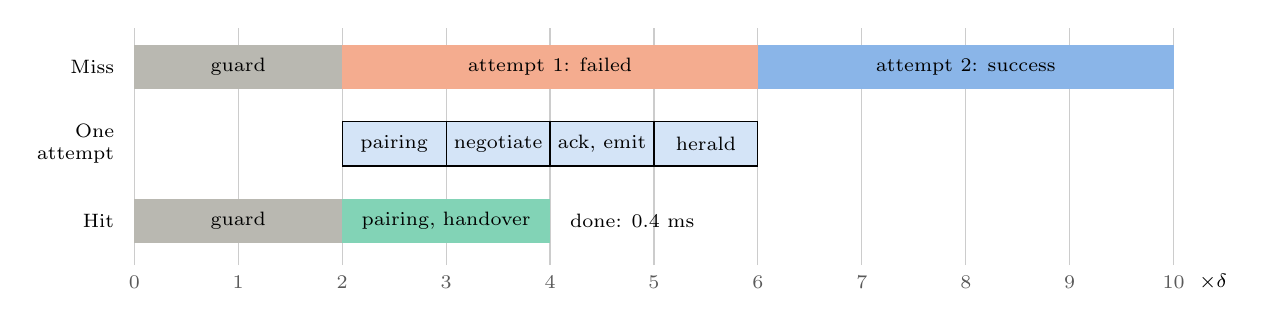
\begin{tikzpicture}[x=13.2mm,y=7mm,font=\scriptsize]
\foreach \i in {0,...,10} {\draw[gray!40] (\i,-0.2) -- (\i,4.1); \node[gray!70!black] at (\i,-0.5) {\i};}
\node[anchor=west] at (10.15,-0.5) {$\times\delta$};
% miss with one failed attempt
\node[anchor=east] at (-0.1,3.4) {Miss};
\fill[guard] (0,3) rectangle (2,3.8); \node at (1,3.4) {guard};
\fill[fail!55] (2,3) rectangle (6,3.8); \node at (4,3.4) {attempt 1: failed};
\fill[demand!55] (6,3) rectangle (10,3.8); \node at (8,3.4) {attempt 2: success};
% one attempt detail
\node[anchor=east,align=right] at (-0.1,2.0) {One\\attempt};
\foreach \a/\b/\t in {2/3/pairing, 3/4/{negotiate}, 4/5/{ack, emit}, 5/6/herald} {\draw[fill=demand!20] (\a,1.6) rectangle (\b,2.4); \node at ({(\a+\b)/2},2.0) {\t};}
% hit
\node[anchor=east] at (-0.1,0.6) {Hit};
\fill[guard] (0,0.2) rectangle (2,1.0); \node at (1,0.6) {guard};
\fill[hit!55] (2,0.2) rectangle (4,1.0); \node at (3,0.6) {pairing, handover};
\node[anchor=west] at (4.1,0.6) {done: 0.4 ms};
\end{tikzpicture}
\caption{Guard is the reservation REQUEST and APPROVE. A failed attempt repeats everything, including pairing. A reverse hop adds one $\delta$ to each attempt and to a hit.}
\end{figure}

\begin{itemize}\setlength{\itemsep}{1pt}
\item \textbf{Hop direction matters.} An attempt takes exactly $4\delta$ (0.4 ms) when the source core number is lower and $5\delta$ (0.5 ms) when it is higher, because the node that sends NEGOTIATE then starts one message later.
\item \textbf{Mean attempts} are $1/p \approx 2.46$. So generation takes 0.98 ms forward and 1.23 ms reverse, about 1.1 ms on average.
\item \textbf{A hit is not free.} It costs 0.4 ms forward or 0.5 ms reverse, with no physical attempts.
\item \textbf{Correction.} Earlier I said ``0.4 ms per attempt''. That holds for only one direction.
\end{itemize}

\section*{4. The knobs}
\begin{table}[H]\centering\small
\begin{tabular}{@{}p{4.0cm}p{4.9cm}p{7.2cm}@{}}\toprule
Knob & Measured effect & Note \\\midrule
Classical delay $\delta$ & scales generation and the guard together & $\times5$ gives 5.44 ms \\
Memory efficiency & changes attempts only & 0.8 gives 1.56 ms, 0.4 gives 5.97 ms \\
Detector efficiency & same as memory efficiency & enters squared \\
BSM success rate & changes attempts only & 0.2 gives 2.64 ms \\
Fibre length & changes both delay and loss & matters at km scale only: 10 km to the BSM gives 5.50 ms \\
Attenuation & changes attempts only & needs $\sim$100 dB/m at 2.5 cm \\
Memory frequency & none at 80 MHz & limits attempts only below about 2 kHz \\
Coherence, raw fidelity, gate and measurement fidelity, gap & no effect on generation time & coherence and raw fidelity change delivered fidelity; at coherence 0.2 ms it is 0.43 \\\bottomrule
\end{tabular}\caption{Single-link results, mean of both hop directions.}\end{table}

\section*{5. Findings so far (interim)}
\textbf{(a) With the 5 ms gap, your idea holds.} Latency gain rises as generation slows.
\begin{table}[H]\centering\small
\begin{tabular}{@{}lrrrrrrr@{}}\toprule
Case, \code{history} & Eff. & ODG (ms) & Dyn. (ms) & Latency & Makespan & Comm. & Hit rate \\\midrule
QFT $M$4 $C$3 & 1.00 & 1.211 & 0.675 & 44.2\% & 11.4\% & 40.9\% & 73.6\% \\
 & 0.95 & 1.322 & 0.703 & 46.8\% & 13.0\% & 43.6\% & 73.6\% \\
 & 0.80 & 1.776 & 0.819 & 53.9\% & 18.0\% & 48.3\% & 73.4\% \\
QAOA $M$4 $C$3 & 0.95 & 1.364 & 0.981 & 28.0\% & 11.4\% & 22.7\% & 53.7\% \\
QAOA $M$3 $C$2 & 0.95 & 1.454 & 1.265 & 13.0\% & 4.9\% & 9.7\% & 38.1\% \\\bottomrule
\end{tabular}\caption{Ten seeds. At baseline, misses come from the planner's memory limit: almost every planned pair arrives in time.}\end{table}

\textbf{(b) A pair waits far longer than it takes to make:} about 1.1 ms to prepare, then about 9 ms in storage, because a two-layer lead usually spans two 5 ms gaps.

\textbf{(c) The most important result so far: Dynamic's advantage depends on that 5 ms gap.}
\begin{table}[H]\centering\small
\begin{tabular}{@{}lrrrrrr@{}}\toprule
QFT $M$3 $C$2, \code{history} & Efficiency & Gap (ms) & ODG (ms) & Dynamic (ms) & Latency gain & Hit rate \\\midrule
Normal generation & 0.95 & 5.0 & 1.357 & 0.933 & +31.3\% & 55.2\% \\
 & 0.95 & 0.5 & 1.357 & 1.472 & $-$8.5\% & 27.4\% \\
 & 0.95 & 0.0 & 1.357 & 1.780 & $-$31.2\% & 16.1\% \\
Slow generation & 0.60 & 5.0 & 3.098 & 1.808 & +41.6\% & 52.4\% \\
 & 0.60 & 0.0 & 3.097 & 3.588 & $-$15.8\% & 17.9\% \\
Very slow generation & 0.40 & 0.0 & 6.722 & 6.752 & $-$0.5\% & 19.7\% \\\bottomrule
\end{tabular}\caption{Four seeds, partial. QAOA $M$3 $C$2 at gap 0 is similar: $-$26.1\% at efficiency 0.95.}\end{table}

This matters because 5 ms is not a physical value. With no gap, default Dynamic is worse than ODG, and a slower generation only reduces how much worse.
So far this is with lead 2 and default options. \textbf{I do not yet know why it gets worse}, or whether better settings fix it. The lead and tuning experiments test that next.

\section*{6. What simulations are running}
One \emph{case} is one setting, for example: QFT, \code{history} route, $M=4$, $C=3$, memory efficiency 0.6.
For each seed, it simulates the whole workload with ODG and again with Dynamic. Each of those is one \emph{simulation}.
Every hop is physically simulated, including every failed attempt, and an audit checks that no physical rule was broken.

\begin{table}[H]\centering\small
\begin{tabular}{@{}rlp{5.0cm}p{5.2cm}r@{}}\toprule
\# & Experiment & What it changes & What it answers & Done \\\midrule
1 & gap (running) & empty-layer gap 0 to 20 ms & how much gain comes from the 5 ms constant & 12/60 \\
2 & efficiency & memory efficiency 1.0 to 0.3, XY and \code{history} & gain against generation time & 40/72 \\
3 & lead\_gap & lead 1 to 8, gap 0 and 5 ms & does a different lead rescue Dynamic? & 0/48 \\
4 & tuning & 27 Dynamic options, one at a time & which knobs truly help & 0/220 \\
5 & delay & classical delay $\times$0.1 to $\times$5 & the same question through $\delta$ & 8/40 \\
6 & memory & $M = 2$ to 8 & how much memory is worth & 1/20 \\
7 & coherence & coherence 1 s to 1 ms & fidelity and pair expiry limits & 0/24 \\
8 & routes & XY, greedy, \code{history}, \code{minhop} & is \code{history} really best at every speed? & 0/24 \\
9 & workloads & Draper, CDKM, random circuit & do results hold on other circuits? & 0/12 \\
10 & chip & fast $\delta$ with short gaps & the chip-scale regime & 0/16 \\
11 & scale & all time constants together & do only ratios matter? & 0/12 \\
12 & equivalence & three causes of the same $p$ & is $p$ one axis? & 0/6 \\
13 & validation & best tuned options on unseen seeds & guards against tuning to noise & later \\\bottomrule
\end{tabular}\caption{Remaining: about 3,100 simulations. Single-link screening is finished, except three reruns.}\end{table}

\textbf{Ten hypotheses} were committed before the sweeps ran, each with a way to fail. They are in the repository at \code{docs/research/}\allowbreak\code{generation-time-2026-11-01/plan.md}, with a logged list of every deviation.

\section*{7. Experiments we could add}
Not running yet. These are options to discuss after the main results.
\begin{itemize}\setlength{\itemsep}{1pt}
\item \textbf{Realistic gap.} Replace the 5 ms constant with a time based on real local-gate durations.
\item \textbf{Slack-aware planner.} Choose the lead from time available in ms, not a fixed layer count. This changes the planner.
\item \textbf{No re-pairing per attempt.} Today a retry repeats pairing. Keeping the pairing would shorten attempts. This changes the protocol.
\item \textbf{Fix the direction effect.} Let the node that starts first act as primary, so every attempt costs $4\delta$.
\item \textbf{Enforce a fidelity threshold.} The trace uses 0.01, so no pair is ever rejected. A real threshold would test Dynamic's storage cost.
\item \textbf{More mappings and circuit seeds,} because each main workload has only one mapping today.
\item \textbf{Torus topology} and \textbf{data teleportation timing,} which are not modelled in this study.
\end{itemize}

\section*{8. Time estimate}
With the Mac awake, plugged in and the other apps closed, cases now take about 2 to 4 minutes.
The experiments should take about \textbf{2.5 to 3.5 hours}. Analysis, figures and the full LaTeX report then take about 1 to 1.5 hours more,
so about \textbf{4 to 5 hours} in total. A closed lid pauses everything, and that time is added on top.
\end{document}
